% vim: ts=4 sts=4 sw=4 et tw=75
\chapter{Design and Implementation}
\label{chap:desipl}
\begin{quote}
    Show me your flowcharts and conceal your tables, and I shall continue
    to be mystified. Show me your tables, and I won't usually need your
    flowcharts; they'll be obvious.
\end{quote}

\begin{quotesrc}
    Frederick P.Brooks, Jr.,\bookname{The Mythical Man Month}
\end{quotesrc}

As the quotation from Brooks's classic book suggests, the design of the
data structures is the central decision in the creation of a program. Once
the data structures are laid out, the algorithms tend to fall into place,
and the coding is comparatively easy.

This point of view is oversimplified but not misleading. In the previous
chapter we examined the basic data structures that are the building blocks
of most programs. In this chapter we will combine such structures as we
work through the design and implementation of a modest-sized program. We
will show how the problem influences the data structures, and how the code
that follows is straightforward once we have the data structures mapped out.

One aspect of this point of view is that the choice of programming Language
is relatively unimportant to the overall design. We will design the
program in the abstract and then write it in C, Java, C++, Awk, and Perl.
Comparing the implementations demonstrates how languages can help or
hinder, and ways in which they are unimportant. Program design can
certainly be colored by a language but is not usually dominated by it.

The problem we have chosen is unusual, but in basic from it is typical of
many programs: some data comes in, some data goes out, and the processing
depends on a little ingenuity.

Specifically, we're going to generate random English text that reads well.
If we emit random letters or random words, the result will be nonsense. For
example, a program that randomly selects letters(and blanks. to separate
words)might produce this:
\begin{wellcode}
    xptmxgn xusaja afqnzgxl lhidwed rjdjuvpydrlwnjy
\end{wellcode}
which is not very convincing. If we weight the letters by their frequency
of appearance in English text, we might get this:
\begin{wellcode}
    idtefoae tcs trder jcii ofdslnqetacp t ola
\end{wellcode}
which isn't a great deal better. Words chosen from the dictionary at random
don't make much more sense:
\begin{wellcode}
    polydactyl equatorial splashily jowl verandah circumscribe
\end{wellcode}
For better results, we need a statistical model with more structure.Such as
the frequency of appearance of whole phrases. But where can we find such
statistics?

We could grab a large body of English and study it in detail, but there is
an easier and more entertaining approach. The key observation is that we
can use any existing text to construct a statistical model of the language
\textit{as used} in \textit{that text}, and from that generate random text
that has similar statistics to the original.

\section{The Markov Chain Algorithm}
\label{sec:the_markov_chain_algorithm}

An elegant way to do this sort of processing is a technique called a
\textit{Markov chain algorithm}. If we imagine the input as a sequence of
overlapping phrases, the algorithm divides each phrase into two parts, a
multi-word \textit{prefix} and a single \textit{suffix} word that follows
the prefix. A Markov chain algorithm emits output phrases by randomly
choosing the suffix that follows the prefix, according to the statistics
of(in our case)the original text. Three-word phrases work well a two-word
prefix is used to select the suffix word:
\\
\indent set \textit{$w_1$} and \textit{$w_2$} to the first two words in the text 
\\
\indent print \textit{$w_1$} and \textit{$w_2$} 
\\
\indent loop:
\\
\indent\indent randomly choose \textit{$w_3$}, one of the successors of
    prefix \textit{$w_1$} \textit{$w_2$} in the text
\\
\indent\indent print \textit{$w_{3}$}
\\
\indent\indent replace \textit{w} and \textit{$w_2$} by \textit{$w_2$} and
        \textit{$w_3$}
\\
\indent\indent repeat loop
\\
To illustrate, suppose we want to generate random text base on a few
sentences paraphrased from the epigraph above, using-word prefixes:
\\
\indent Show your flowcharts and conceal your tables and I will be
mystified. Show your tables and you flowcharts will be obvious.\textit{(end)}
\\
These are some of the pairs of input words and the words that follow them:
\\
\indent \begin{tabular}{ll}
    \textit{Input prefix:} & \textit{Suffix words that follow:}\\
    Show your & flowcharts tables\\
    your flowcharts & and will\\
    flowcharts and & conceal\\
    flowcharts will & be\\
    your tables & and and\\
    will be & mystified. obvious.\\
    be mystified. & Show\\
    be obvious. & \textit{(end)}
\indent \end{tabular} \\
A Markov algorithm processing this text will begin by printing \textit{Show
    your} and will then randomly pick either \textit{flowcharts} or
\textit{tables}. If it choose the former, the current prefix becomes
\textit{your flowcharts} and next word will be \textit{and} or
\textit{will}. If it chooses \textit{tables}, the next word will be
\textit{and}. This continues until enough output has been generated or
until the end-marker is encountered as a suffix.

Our program will read a piece of English text and use a Markov chain
algorithm to generate new text based on the frequency of appearance of
phrases of a fixed length. The number of words in the prefix, which is two
in our example, is a parameter. Making the prefix shorter tends to produce
less coherent prose; making it longer tends to reproduce the input text
verbatim. For English text, using two words to select a third is a good
compromise; it seems to recreate the flavor of the input while adding its
own whimsical touch.

What is a word? The obvious answer is a sequence of alphabetic characters,
but it is desirable to leave punctuation attached to the words so
\textit{"words"} and \textit{"words."} are different. This helps to improve
the quality of the generated prose by letting punctuation, and
therefore(indirectly)grammar, influence the word choice, although it also
permits unbalanced quotes and parentheses to sneak in. We will therefore
define a "word" as anything between white space, a decision that places no
\textit{restriction} on input language and leaves punctuation attached to
the words. Since most programming languages have facilities to split text
into white-space-separated words, this is also easy to implement.

Because of the method, all words, all two-word phrases, and all three-word
phrases in the output must have appeared in the input, but there should be
many four-word and longer phrases that are synthesized. Here are a few
sentences produced by the program we will develop in this chapter, when
given the text of Chapter VII of
\bookname{The Sun Also Rises} by Ernest Hemingway:
\begin{oldquote}
    As I started up the undershirt onto his chest black, and big stomach
    muscles bulging under the light. "You see them?" Below the line where
    his ribs stopped were two raised white welts. "See on the forehead."
    "Oh, Brett, I love you." "Let's not talk. Talking's all bilge. I'm
    going away tomorrow." "Tomorrow?" "Yes. Didn't I say so? I am." "Let's
    have a drink, then."
\end{oldquote}

We were lucky here that punctuation (标点符号) came out correctly; that
need not happen.

\section{Data Structure Alternatives}
\label{sec:data_structure_alternatives}

How much input do we intend to deal with? How fast must the program run? It
seems reasonable to ask our program to read in a whole book, so we should
be prepared for input sizes of $n = 100,000$ words or more. The output will
be hundreds or perhaps thousands of words, and the program should run in a
few seconds instead of minutes. With 100,000 words of input text, $n$ is
fairly large so the algorithms can't be too simplistic if we want the
program to be fast.

The Markov algorithm must see all the input before it can begin to generate
output, so it must store the entire input in some form. One possibility is
to read the whole input and store it in a long string, but we clearly want
the input broken down into words. If we store it as an array of pointers to
words, output generation is simple: to produce each word, scan the input
text to see what possible suffix words follow the prefix that was just
emitted, and then choose one at random. However, that means scanning all
100,000 input words for each word we generate; 1,000 words of output means
hundreds of millions of string comparisons, which will not be fast.

Another possibility is to store only unique input words, together with a
list of where they appear in the input so that we can locate successor
words more quickly.  We could use a hash table like the one in Chapter
\ref{chap:alds}, but that version doesn't directly address the needs of the
Markov algorithm, which must quickly locate all the suffixes of a given
prefix.

We need a data structure that better represents a prefix and its associated
suffixes.  The program will have two passes, an input pass that builds the
data structure representing the phrases, and an output pass that uses the
data structure to generate the random output. In both passes, we need to
look up a prefix (quickly): in the input pass to update its suffixes, and
in the output pass to select at random from the possible suffixes. This
suggests a hash table whose keys are prefixes and whose values are the sets
of suffixes for the corresponding prefixes.

For purposes of description, we'll assume a two-word prefix, so each output
word is based on the pair of words that precede it. The number of words in
the prefix doesn't affect the design and the programs should handle any
prefix length, but selecting a number makes the discussion concrete. The
prefix and the set of all its possible suffixes we'll call a state, which
is standard terminology for Markov algorithms.

Given a prefix, we need to store all the suffixes that follow it so we can
access them later. The suffixes are unordered and added one at a time. We
don't know how many there will be, so we need a data structure that grows
easily and efficiently, such as a list or a dynamic array. When we are
generating output, we need to be able to choose one suffix at random from
the set of suffixes associated with a particular prefix. Items are never
deleted.

What happens if a phrase appears more than once? For example, 'might appear
twice' might appear twice but 'might appear once' only once. This could be
represented by putting 'twice' twice in the suffix list for 'might appear'
or by putting it in once, with an associated counter set to 2. We've tried
it with and without counters; without is easier, since adding a suffix
doesn't require checking whether it's there already, and experiments showed
that the difference in run-time was negligible (可以忽略的).

In summary, each state comprises (包含) a prefix and a list of suffixes.
This information is stored in a hash table, with prefix as key. Each prefix
is a fixed-size set of words.  If a suffix occurs more than once for a
given prefix, each occurrence will be included separately (单独地) in the
list.

The next decision is how to represent the words themselves. The easy way is
to store them as individual strings. Since most text has many words
appearing multiple times, it would probably save storage if we kept a
second hash table of single words, so the text of each word was stored only
once. This would also speed up hashing of prefixes, since we could compare
pointers rather than individual characters: unique strings have unique
addresses. We'll leave that design as an exercise; for now, strings will be
stored individually.

\section{Building the Data structure in C}
\label{sec:building_the_data_structure_in_c}

Let's begin with a C implementation. The first step is to define some
constants.
\begin{wellcode}
    enum {
        NPREF   = 2,        /* number of prefix words */
        NHASH   = 4093,     /* size of state hash table array */
        MAXGEN  = 10000     /* maximum words generated */
    };
\end{wellcode}
This declaration defines the number of words (\verb'NPREF') for the prefix,
the size of the hash table array (\verb'NHASH'), and an upper limit on the
number of words to generate (\verb'MAXGEN'). If \verb'NPREF' is a
compile-time constant rather than a run-time variable, storage management
is simpler. The array size is set fairly large because we expect to give
the program large input documents, perhaps a whole book. We chose
\verb'NHASH = 4093' so that if the input has 10,000 distinct prefixes (word
pairs), the average chain will be very short, two or three prefixes. The
larger the size, the shorter the expected length of the chains and thus the
faster the lookup. This program is really a toy, so the performance isn't
critical, but if we make the array too small the program will not handle
our expected input in reasonable time; on the other hand, if we make it too
big it might not fit in the available memory.

The prefix can be stored as an array of words. The elements of the hash
table will be represented as a \verb'State' data type, associating the
\verb'Suffix' list with the prefix:
\begin{wellcode}
    typedef struct State State;
    typedef struct Suffix Suffix;
    struct State {  /* prefix + suffix list */
        char    *pref[NPREF];   /* prefix words */
        Suffix  *suf;           /* list of suffixes */
        State   *next;          /* next in hash table */
    };

    struct Suffix { /* list of suffixes */
        char    *word;  /* suffix */
        Suffix  *next;  /* next in list of suffixes */
    };

    State   *statetab[NHASH];   /* hash table of states */
\end{wellcode}
Pictorially (形象地), the data structures look like this:

\begin{center}
    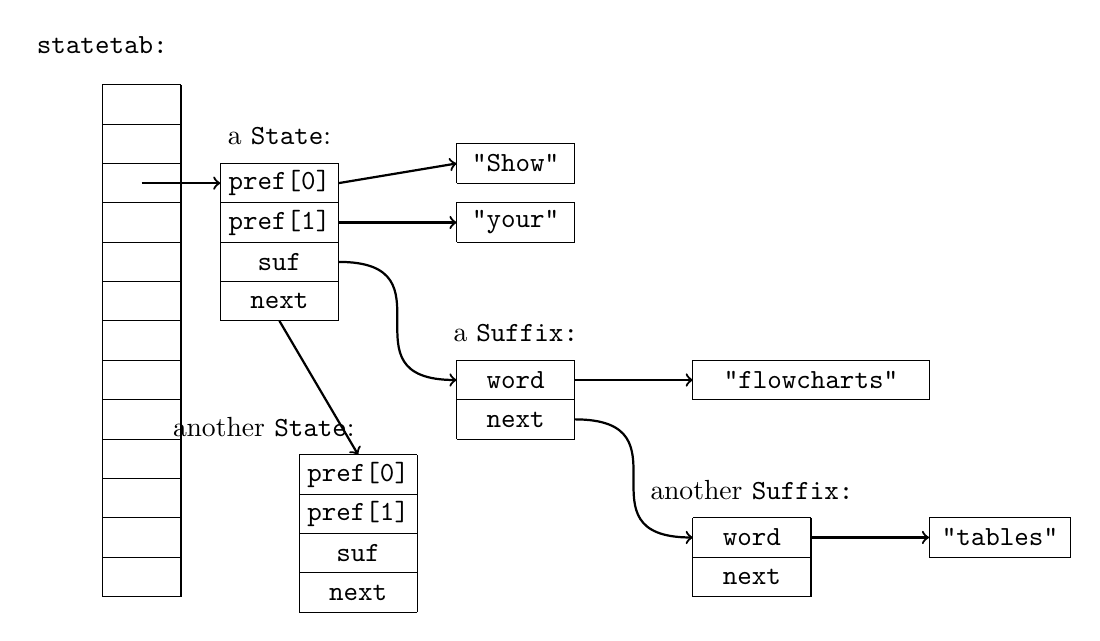
\begin{tikzpicture}
        \pgfmathsetmacro\width{1.0};
        \pgfmathsetmacro\height{0.5};

        \draw (0, 0) -- (0, 13 * \height);
        \draw (0 + \width, 0) -- (0 + \width, 13 * \height);
        \foreach \i in {0,...,13}
            \draw (0, \i * \height) -- (0 + \width, \i * \height);
        \node at (0, 14 * \height) {\verb'statetab:'};

        % a State
        \draw[thick, ->] (\width / 2, \height * 10.5) --
            (\width / 2 + 1.0, \height * 10.5);
        \draw (\width / 2 + 1.0, 7.0 * \height) -- (\width / 2 + 1.0,
            11.0 * \height);
        \draw (\width / 2 + 2.5, 7.0 * \height) -- (\width / 2 + 2.5,
            11.0 * \height);
        \foreach \i in {0,...,4}
            \draw (\width / 2 + 1.0, 7.0 * \height + \i * \height) --
                (\width / 2 + 2.5, 7.0 * \height + \i * \height);
        \node at (\width / 2 + 1.75, 7.5 * \height)
            {\verb'next'};
        \node at (\width / 2 + 1.75, 7.5 * \height + \height)
            {\verb'suf'};
        \node at (\width / 2 + 1.75, 7.5 * \height + 2 * \height)
            {\verb'pref[1]'};
        \node at (\width / 2 + 1.75, 7.5 * \height + 3 * \height)
            {\verb'pref[0]'};
        \node at (\width / 2 + 1.75, 7.5 * \height + 4.2 * \height)
            {a \verb'State':};

        % another State
        \draw[thick, ->] (\width / 2 + 1.75, 7 * \height) --
            (\width / 2 + 2.75, 7.0 * \height - 1.7);
        \draw (\width / 2 + 2.0, 3.0 * \height - 1.7) --
            (\width / 2 + 2.0, 7.0 * \height - 1.7);
        \draw (\width / 2 + 3.5, 3.0 * \height - 1.7) --
            (\width / 2 + 3.5, 7.0 * \height - 1.7);
        \foreach \i in {0,...,4}
            \draw (\width / 2 + 2.0, 3.0 * \height - 1.7 + \i * \height) --
                (\width / 2 + 3.5, 3.0 * \height - 1.7 + \i * \height);
        \node at (\width / 2 + 2.75, 3.5 * \height - 1.7)
            {\verb'next'};
        \node at (\width / 2 + 2.75, 3.5 * \height + \height - 1.7)
            {\verb'suf'};
        \node at (\width / 2 + 2.75, 3.5 * \height + 2 * \height - 1.7)
            {\verb'pref[1]'};
        \node at (\width / 2 + 2.75, 3.5 * \height + 3 * \height - 1.7)
            {\verb'pref[0]'};
        \node at (\width / 2 + 1.55, 3.5 * \height + 4.2 * \height - 1.7)
            {another \verb'State':};

        % "Show" and "your"
        \draw[thick, ->] (\width / 2 + 2.5, 9.5 * \height) --
            (\width / 2 + 4.0, 9.5 * \height);
        \draw[thick, ->] (\width / 2 + 2.5, 10.5 * \height) --
            (\width / 2 + 4.0, 11 * \height);
        \draw (\width / 2 + 4.0, 9.0 * \height) -- (\width / 2 + 4.0,
            10.0 * \height) -- (\width / 2 + 5.5, 10.0 * \height) --
            (\width / 2 + 5.5, 9.0 * \height) --
            (\width / 2 + 4.0, 9.0 * \height);
        \draw (\width / 2 + 4.0, 9.0 * \height + 0.75) --
            (\width / 2 + 4.0, 10.0 * \height + 0.75) --
            (\width / 2 + 5.5, 10.0 * \height + 0.75) --
            (\width / 2 + 5.5, 9.0 * \height + 0.75) --
            (\width / 2 + 4.0, 9.0 * \height + 0.75);
        \node at (\width / 2 + 4.75, 9.5 * \height) {\verb'"your"'};
        \node at (\width / 2 + 4.75, 11.0 * \height) {\verb'"Show"'};

        % a Suffix
        \draw[thick, ->] (\width / 2 + 2.5, 8.5 * \height)
            .. controls (\width / 2 + 4.0, 8.5 * \height) and
            (\width / 2 + 2.5, 8.5 * \height - 1.5) ..
            (\width / 2 + 4.0, 8.5 * \height - 1.5);
        \draw (\width / 2 + 4.0, 6 * \height) --
            (\width / 2 + 4.0, 4 * \height);
        \draw (\width / 2 + 5.5, 6 * \height) --
            (\width / 2 + 5.5, 4 * \height);
        \foreach \i in {0,...,2}
            \draw (\width / 2 + 4.0, 4.0 * \height + \i * \height) --
                (\width / 2 + 5.5, 4.0 * \height + \i * \height);
        \node at (\width / 2 + 4.75, 4.5 * \height) {\verb'next'};
        \node at (\width / 2 + 4.75, 5.5 * \height) {\verb'word'};
        \node at (\width / 2 + 4.75, 6.7 * \height) {a \verb'Suffix:'};

        % "flowcharts"
        \draw[thick, ->] (\width / 2 + 5.5, 5.5 * \height) --
            (\width / 2 + 7.0, 5.5 * \height);
        \draw (\width / 2 + 7.0, 5.0 * \height) --
            (\width / 2 + 7.0, 6.0 * \height) --
            (\width / 2 + 10, 6.0 * \height) --
            (\width / 2 + 10, 5.0 * \height) --
            (\width / 2 + 7.0, 5.0 * \height);
        \node at (\width / 2 + 8.5, 5.5 * \height) {\verb'"flowcharts"'};

        % another Suffix
        \draw[thick, ->] (\width / 2 + 5.5, 4.5 * \height) ..
            controls (\width / 2 + 7.0, 4.5 * \height) and
            (\width / 2 + 5.5, 1.5 * \height) ..
            (\width / 2 + 7.0, 1.5 * \height);
        \draw (\width / 2 + 7.0, 2.0 * \height) --
            (\width / 2 + 7.0, 0);
        \draw (\width / 2 + 8.5, 2.0 * \height) --
            (\width / 2 + 8.5, 0);
        \foreach \i in {0,...,2}
            \draw (\width / 2 + 7.0, \i * \height) --
                (\width / 2 + 8.5, \i * \height);
        \node at (\width / 2 + 7.75, 0.5 * \height) {\verb'next'};
        \node at (\width / 2 + 7.75, 1.5 * \height) {\verb'word'};
        \node at (\width / 2 + 7.75, 2.7 * \height)
            {another \verb'Suffix:'};

        % "tables"
        \draw[thick, ->] (\width / 2 + 8.5, 1.5 * \height) --
            (\width / 2 + 10, 1.5 * \height);
        \draw (\width / 2 + 10, \height) -- (\width / 2 + 10, 2 * \height)
        -- (\width / 2 + 11.8, 2 * \height) --
        (\width / 2 + 11.8, \height) -- (\width / 2 + 10, \height);
        \node at (\width / 2 + 10.9, 1.5 * \height) {\verb'"tables"'};
    \end{tikzpicture}
\end{center}

We need a hash function for prefixes, which are arrays of strings. It is
simple to modify the string hash function \verb'fmm' Chapter
\ref{chap:alds} to loop over the strings in the array, thus in effect
hashing the concatenation of the strings:
\begin{wellcode}
    /* hash: compute hash value for array of NPREF strings */
    unsigned int hash(char *s[NPREF])
    {
        unsigned int    h;
        unsigned char   *p;
        int i;

        h = 0;
        for (i = 0; i < NPREF; i++)
            for (p = (unsigned char *)s[i]; *p != '\0'; p++)
                h = MULTIPLIER * h + *p;
        return h % NHASH;
    }
\end{wellcode}

A similar modification to the \verb'lookup' routine completes the
implementation of the hash table:
\begin{wellcode}
    /* lookup: search for prefix; create if requested. */
    /* return pointer if present or created; NULL if not */
    /* creation doesn't strdup so strings mustn't change later */
    State *lookup(char *prefix[NPREF], int create)
    {
        int i, h;
        State *sp;

        h = hash(prefix);
        for (sp = statetab[h]; sp != NULL; sp = sp->next) {
            for (i = 0; i < NPREF; i++)
                if (strcmp(prefix[i], sp->pref[i]) != 0)
                    break;
            for (i == NPREF)    /* found it */
                return sp;
        }
        if (create) {
            sp = (State *)emalloc(sizeof(State));
            for (i = 0; i < NPREF; i++)
                sp->pref[i] = prefix[i];
            sp->suf = NULL;
            sp->next = statetab[h];
            statetab[h] = sp;
        }
        return sp;
    }
\end{wellcode}

Next we need to build the hash tables as the file is read:
\begin{wellcode}
    /* build: read input, build prefix table */
    void build(char *prefix[NPREF], FILE *f)
    {
        char    buf[100], fmt[10];

        /* create a format string; %s could overflow buf */
        sprintf(fmt, "%%%ds", sizeof(buf) - 1);
        while (fscanf(f, fmt, buf) != EOF)
            add(prefix, estrdup(buf));
    }
\end{wellcode}

The peculiar (罕见的) call to \verb'sprintf' gets around an irritating
(气人的) problem with \verb'fscanf', which is otherwise perfect for the
job. A call to \verb'fscanf' with format \verb'%s' will read the next
white-space-delimited word from the file into the buffer, but there is no
limit on size: a long word might overflow the input buffer, wreaking havoc
(报复性地破坏). If the buffer is 100 bytes long (which is far beyond what
we expect ever to appear in normal text), we can use the format \verb'%99s'
(leaving one byte for the terminal \verb"'\0'"), which tells \verb'fscanf'
to stop after 99 bytes. A long word will be broken into pieces, which is
unfortunate but safe. We could declare
\begin{badcode}
    enum { BUFSIZE = 100 };
    char    fmt[] = "%99s"; /* BUFSIZE - 1 */
\end{badcode}
but that requires two constants for one arbitrary decision -- the size of
the buffer -- and introduces the need to maintain their relationship. The
problem can be solved once and for all by creating the format string
dynamically with \verb'sprintf', so that's the approach we take.

The two arguments to build are the prefix array holding the previous
\verb'NPREF' words of input and a \verb'FILE' pointer. It passes the prefix
and a copy of the input word to add, which adds the new entry to the hash
table and advances the prefix:
\begin{wellcode}
    /* add: add word to suffix list, update the prefix */
    void add(char *prefix[NPREF], char *suffix)
    {
        State   *sp;

        sp = lookup(prefix, 1); /* create if not found */
        addsufix(sp, suffix);
        /* move the words down the prefix */
        memmove(prefix, prefix+1, (NPREF-1)*sizeof(prefix[0]));
        prefix[NPREF-1] = suffix;
    }
\end{wellcode}

The call to \verb'memmove' is the idiom for deleting from an array. It
shifts elements \verb'1' through \verb'NPREF-1' in the prefix down to
positions \verb'0' through \verb'NPREF-2', deleting the first prefix word
and opening a space for a new one at the end.

The \verb'addsuffix' routine adds the new suffix:
\begin{wellcode}
    /* addsuffix: add to state. suffix must not change later */
    void addsuffix(State *sp, char *suffix)
    {
        Suffix  *suf;

        suf = (Suffix *)emalloc(sizeof(Suffix));
        suf->word = suffix;
        suf->next = sp->suf;
        sp->suf = suf;
    }
\end{wellcode}
We split the action of updating the state into two functions: \verb'add'
performs the general service of adding a suffix to a prefix, while
\verb'addsuffix' performs the implementation-specific action of adding a
word to a suffix list. The \verb'add' routine is used by \verb'build', but
\verb'addsuffix' is used internally only by \verb'add'; it is an
implementation detail that might change and it seems better to have it in a
separate function, even though it is called in only one place.

\section{Generating Output}
\label{sec:generating_output}

With the data structure built, the next step is to generate the output. The
basic idea is as before: given a prefix, select one of its suffixes at
random, print it, then advance the prefix. This is the steady (稳定的)
state of processing; we must still figure out how to start and stop the
algorithm. Starting is easy if we remember the words of the first prefix
and begin with them. Stopping is easy, too. We need a marker word to
terminate the algorithm. After all the regular input, we can add a
terminator, a "word" that is guaranteed not to appear in any input:
\begin{wellcode}
    build(prefix, stdin);
    add(prefix, NONWORD);
\end{wellcode}
\verb'NONWORD' should be some value that will never be encountered in
regular input. Since the input words are delimited by white space, a "word"
of white space will serve, such as a newline character:
\begin{wellcode}
    char    NONWORD[] = '\n';   /* cannot appear as read word */
\end{wellcode}

One more worry: what happens if there is insufficient input to start the
algorithm?  There are two approaches to this sort of problem, either exit
prematurely if there is insufficient input, or arrange that there is always
enough and don't bother to check.  In this program, the latter approach
works well.

We can initialize building and generating with a fabricated (伪造的)
prefix, which guarantees there is always enough input for the program. To
prime (启动) the loops, initialize the prefix array to be all
\verb'NONWORD' words. This has the nice benefit that the first word of the
input file will be the first suffix of the fake prefix, so the generation
loop needs to print only the suffixes it produces.

In case the output is unmanageably long, we can terminate the algorithm
after some number of words are produced or when we hit \verb'NONWORD' as a
suffix, whichever comes first.

Adding a few \verb'NONWORD's to the ends of the data simplifies the main
processing loops of the program significantly; it is an example of the
technique of adding sentinel (哨兵) values to mark boundaries.

As a rule, try to handle irregularities and exceptions and special cases in
data.
Code is harder to get right so the control flow should be as simple and
regular as possible.

The \verb'generate' function uses the algorithm we sketched (描绘的)
originally. It produces one word per line of output, which can be grouped
into longer lines with a word processor; Chapter \ref{chap:notation} shows
a simple formatter called \verb'fmt'for this task.

With the use of the initial and final \verb'NONWORD' strings,
\verb'generate' starts and stops properly:
\begin{wellcode}
    /* generate: produce output, one word per line */
    void generate(int nwords)
    {
        State   *sp;
        Suffix  *suf;
        char    *prefix[NPREF], *w;
        int     i, nmatch;

        for (i = 0; i < NPREF; i++) /* reset initial prefix */
            prefix[i] = NONWORD;

        for (i = 0; i < nwords; i++) {
            sp = lookup(prefix, 0);
            nmatch = 0;
            for (suf = sp->suf; suf != NULL; suf = suf->next)
                if (rand() % ++nmatch == 0) /* prob = 1/nmatch */
                    w = suf->word;
            if (strcmp(w, NONWORD) == 0)
                break;
            printf("%s\n", w);
            memmove(prefix, prefix+1, (NPREF-1)*sizeof(prefix[0]));
            prefix[NPREF-1] = w;
        }
    }
\end{wellcode}

Notice the algorithm for selecting one item at random when we don't know
how many items there are. The variable \verb'nmatch' counts the number of
matches as the list is scanned. The expression
\begin{wellcode}
    rand() % ++nmatch == 0
\end{wellcode}
increments \verb'nmatch' and is then true with probability \verb'1/nmatch'.
Thus the first matching item is selected with probability 1, the second
will replace it with probability $1/2$, the third will replace the survivor
with probability $1/3$, and so on. At any time, each one of the $k$
matching items seen so far has been selected with probability $1/k$.

At the beginning, we set the \verb'prefix' to the starting value, which is
guaranteed to be installed in the hash table. The first \verb'Suffix'
values we find will be the first words of the document, since they are the
unique follow-on to the starting prefix. After that, random suffixes will
be chosen. The loop calls \verb'lookup' to find the hash table entry for
the current prefix, then chooses a random suffix, prints it, and advances
the \verb'prefix'.

If the suffix we choose is \verb'NONWORD', we're done, because we have
chosen the state that corresponds to the end of the input. If the suffix is
not \verb'NONWORD', we print it, then drop the first word of the prefix
with a call to \verb'memmove', promote the suffix to be the last word of
the prefix, and loop.

Now we can put all this together into a \verb'main' routine that reads the
standard input and generates at most a specified number of words:
\begin{wellcode}
    /* markov main: markov-chain random text generation */
    int main(void)
    {
        int i, nwords = MAXGEN;
        char    *prefix[NPREF];     /* current input prefix */
        for (i = 0; i < NPREF; i++) /* set up initial prefix */
            prefix[i] = NONWORD;
        build(prefix, stdin);
        add(prefix, NONWORD);
        generate(nwords);
        return 0;
    }
\end{wellcode}

This completes our C implementation. We will return at the end of the
chapter to a comparison of programs in different languages. The great
strengths of C are that it gives the programmer complete control over
implementation, and programs written in it tend to be fast. The cost,
however, is that the C programmer must do more of the work, allocating and
reclaiming memory, creating hash tables and linked lists, and the like. C
is a razor-sharp tool, with which one can create an elegant and efficient
program or a bloody mess.

\begin{exercise}
    The algorithm for selecting a random item from a list of unknown length
    depends on having a good random number generator. Design and carry out
    experiments to determine how well the method works in practice.
\end{exercise}

\begin{exercise}
    If each input word is stored in a second hash table, the text is only
    stored once, which should save space. Measure some documents to
    estimate how much. This organization would allow us to compare pointers
    rather than strings in the hash chains for prefixes, which should run
    faster. Implement this version and measure the change in speed and
    memory consumption.
\end{exercise}

\begin{exercise}
    Remove the statements that place sentinel \verb'NONWORD's at the
    beginning and end of the data, and modify \verb'generate' so it starts
    and stops properly without them. Make sure it produces correct output
    for input with 0, 1, 2, 3, and 4 words.  Compare this implementation to
    the version using sentinels.
\end{exercise}

\section{Java}
\label{sec:java}

Our second implementation of the Markov chain algorithm is in Java.
Object-oriented languages like Java encourage one to pay particular
attention to the interfaces between the components of the program, which
are then encapsulated as independent data items called objects or classes,
with associated functions called methods.

Java has a richer library than C, including a set of \textit{container}
classes to group existing objects in various ways. One example is a
\verb'Vector' that provides a dynamically-growable array that can store any
Object type. Another example is the \verb'Hashtable' class, with which one
can store and retrieve values of one type using objects of another type as
keys.

In our application, \verb'Vectors' of strings are the natural choice to
hold prefixes and suffixes. We can use a \verb'Hashtable' whose keys are
prefix vectors and whose values are suffix vectors. The terminology for
this type of construction is a map from prefixes to suffixes; in Java, we
need no explicit \verb'State' type because \verb'Hashtable' implicitly
connects (maps) prefixes to suffixes. This design is different from the C
version, in which we installed \verb'State' structures that held both
prefix and suffix list, and hashed on the prefix to recover the full
\verb'State'.

A \verb'Hashtable' provides a \verb'put' method to store a key-value pair,
and a \verb'get' method to retrieve the value of a key:
\begin{wellcode}
    Hashtable h = new Hashtable();
    h.put(key, value);
    Sometype v = (Sometype)h.get(key);
\end{wellcode}

Our implementation has three classes. The first class \verb'Prefix', holds
the words of the prefix:
\begin{wellcode}
    class Prefix {
        public Vector pref; // NPREF adjacent words from input
        ...
\end{wellcode}

The second class, \verb'Chain', reads the input, builds the hash table, and
generates the output; here are its class variables:
\begin{wellcode}
    class Chain {
        static final int NPREF  = 2;    // size of prefix
        static final String NONWORD = "\n";
                    // "word" that can't appear
        Hashtable statetab = new Hashtable();
                    // key = Prefix, value = suffix Vector
        Prefix prefix = new Prefix(NPREF, NONWORD);
                    // initial prefix
        Random rand = new Random();
        ...
\end{wellcode}

The third class is the public interface; it holds \verb'main' and
instantiates a \verb'Chain':
\begin{wellcode}
    class Markov {
        static final int MAXGEN = 10000; // maximum words generated
        public static void main(String[] args) throws IOException
        {
            Chain chain = new Chain();
            int nwords = MAXGEN;

            chain.build(System.in);
            chain.generate(nwords);
        }
    }
\end{wellcode}

When an instance of class \verb'Chain' is created, it in turn creates a
hash table and sets up the initial prefix of \verb'NPREF' \verb'NONWORD's.
The \verb'build' function uses the library function \verb'StreamTokenizer'
to parse the input into words separated by white space characters.  The
three calls before the loop set the tokenizer into the proper state for our
definition of "word".
\begin{wellcode}
    // Chain build: build State table from input stream
    void build(InputStream in) throws IOException
    {
        StreamTokenizer st = new StreamTokenizer(in);

        st.resetSyntax();                     // remove default rules
        st.wordChars(0, Character.MAX_VALUE); // turn on all chars
        st.whitespaceChar(0, ' ');            // except up to blank
        while (st.nextToken() != st.TT_EOF)
            add(st.sval);
        add(NONWORD);
    }
\end{wellcode}

The \verb'add' function retrieves the vector of suffixes for the current
prefix from the hash table; if there are none (the vector is null),
\verb'add' creates a new vector and a new prefix to store in the hash
table. In either case, it adds the new word to the suffix vector and
advances the prefix by dropping the first word and adding the new word at
the end.
\begin{wellcode}
    // Chain add: add word to suffix list, update prefix
    void add(String word)
    {
        Vector suf = (Vector)statetab.get(prefix);
        if (suf == null) {
            suf = new Vector();
            statetab.put(new Prefix(prefix), suf);
        }
        suf.addElement(word);
        prefix.pref.removeElementAt(0);
        prefix.pref.addElement(word);
    }
\end{wellcode}
Notice that if \verb'suf' is null, \verb'add' installs a new \verb'Prefix'
in the hash table, rather than \verb'prefix' itself. This is because the
\verb'Hashtable' class stores items by reference, and if we don't make a
copy, we could overwrite data in the table. This is the same issue that we
had to deal with in the C program.

The \verb'generation' function is similar to the C version, but slightly
more compact because it can index a random vector element directly instead
of looping through a list.
\begin{wellcode}
    // Chain generate: generate output words
    void generate(int nwords)
    {
        prefix = new Prefix(NPREF, NONWORD);
        for (int i = 0; i < nwords; i++) {
            Vector s = (Vector)statetab.get(prefix);
            int r = Math.abs(rand.nextInt() % s.size());
            String suf = (String)s.elementAt(r);
            if (suf.equals(NONWORD))
                break;
            System.out.println(suf);
            prefix.pref.removeElementAt(0);
            prefix.pref.addElement(suf);
        }
    }
\end{wellcode}

The two constructors of \verb'Prefix' create new instances from supplied
data. The first copies an existing \verb'Prefix', and the second creates a
prefix from \verb'n' copies of a string; we use it to make \verb'NPREF'
copies of \verb'NONWORD' when initializing:
\begin{wellcode}
    // Prefix constructor: duplicate existing prefix
    Prefix (Prefix p)
    {
        pref = (Vector)p.pref.clone();
    }

    // Prefix constructor: n copies of str
    Prefix(int n, String str)
    {
        pref = new Vector();
        for (int i = 0; i < n; i++)
            pref.addElement(str);
    }
\end{wellcode}

\verb'Prefix' also has two methods, \verb'hashCode' and \verb'equals', that
are called implicitly by the implementation of \verb'Hashtable' to index
and search the table. It is the need to have an explicit class for these
two methods for \verb'Hashtable' that forced us to make \verb'Prefix' a
full-fledged (发育完全的) class, rather than just a \verb'Vector' like the
suffix.

The \verb'hashCode' method builds a single hash value by combining the set
of \verb'hashCode's for the elements of the vector:
\begin{wellcode}
    static final int MULTIPLIER = 31;   // for hashCode()

    // Prefix hashCode: generate hash from all prefix words
    public int hashCode()
    {
        int h = 0;
        for (int i = 0; i < pref.size(); i++)
            h = MULTIPLIER * h + pref.elementAt(i).hashCode();
        return h;
    }
\end{wellcode}
and \verb'equals' does an elementwise comparison for the words in two
prefixes:
\begin{wellcode}
    // Prefix equals: compare two prefixes for equal words
    public boolean equals(Object o)
    {
        Prefix p = (Prefix)o;
        for (int i = 0; i < pref.size(); i++)
            if (!pref.elementAt(i).equals(p.pref.elementAt(i)))
                return false;
        return true;
    }
\end{wellcode}

The Java program is significantly smaller than the C program and takes care
of more details; \verb'Vectors' and the \verb'Hashtable' are the obvious
examples. In general, storage management is easy since vectors grow as
needed and garbage collection takes care of reclaiming memory that is no
longer referenced. But to use the \verb'Hashtable' class, we still need to
write functions \verb'hashcode' and \verb'equals', so Java isn't taking
care of all the details.

Comparing the way the C and Java programs represent and operate on the same
basic data structure, we see that the Java version has better separation of
functionality.  For example, to switch from \verb'Vectors' to arrays would
be easy. In the C version, everything knows what everything else is doing:
the hash table operates on arrays that are maintained in various places,
\verb'lookup' knows the layout of the \verb'State' and \verb'Suffix'
structures, and everyone knows the size of the \verb'prefix' array.
\begin{wellcode}
    % java Markov < jr_chemistry.txt | fmt
    Wash the blackboard. Watch it dry. The water goes
    into the air. When water goes into the air it
    evaporates. Tie a damp cloth to one end of a solid or
    liquid. Look around. What are the solid things?
    Chemical changes take place when something burns. If
    the burning material has liquids, they are stable and
    burning. Break up the lump of sugar into small pieces
    and put them together again in the bottom of a liquid.
\end{wellcode}

\begin{wellcode}
    Revise the Java version of \verb'markov' to use an array instead of a
    \verb'Vector' for the prefix in the \verb'State' class.
\end{wellcode}

\section{C++}
\label{sec:c++}

Our third implementation is in C++. Since C++ is almost a superset of C, it
can be used as if it were C with a few notational conveniences, and our
original C version of \verb'markov' is also a legal C++ program. A more
appropriate use of C++, however, would be to define classes for the objects
in the program, more or less as we did in Java; this would let us hide
implementation details. We decided to go even further by using the Standard
Template Library or STL, since the STL has built-in mechanisms that will do
much of what we need. The IS0 standard for C++ includes the STL as part of
the language definition.

The STL provides containers such as vectors, lists, and sets, and a family
of fundamental algorithms for searching, sorting, inserting, and deleting.
Using the template features of C++, every STL algorithm works on a variety
of containers, including both user-defined types and built-in types like
integers. Containers are expressed as C++ templates that are instantiated
for specific data types; for example, there is a \verb'vector' container
that can be used to make particular types like \verb'vector<int>' or
\verb'vector<string>'. All \verb'vector' operations, including standard
algorithms for sorting, can be used on such data types.

In addition to a \verb'vector' container that is similar to Java's
\verb'Vector', the STL provides a \verb'deque' container. A \verb'deque'
(pronounced "deck") is a double-ended queue that matches what we do with
prefixes: it holds \verb'NPREF' elements, and lets us pop the first element
and add a new one to the end, in $O(1)$ time for both. The STL \verb'deque'
is more general than we need, since it permits push and pop at either end,
but the performance guarantees make it an obvious choice.

The STL also provides an explicit \verb'map' container, based on balanced
trees, that stores key-value pairs and provides $O(\log n)$ retrieval of
the value associated with any key. Maps might not be as efficient as $O(1)$
hash tables, but it's nice not to have to write any code whatsoever
(无论什么) to use them. (Some non-standard C++ libraries include a
\verb'hash' or \verb'hash_map' container whose performance may be better.)

We also use the built-in comparison functions, which in this case will do
string comparisons using the individual strings in the prefix.

With these components in hand, the code goes together smoothly. Here are
the declarations:
\begin{wellcode}
    typedef deque<string> Prefix;
    map<Prefix, vector<string>> statetab; // prefix -> suffixes
\end{wellcode}

The STL provides a template for deques; the notation \verb'deque<string>'
specializes it to a deque whose elements are strings. Since this type
appears several times in the program, we used a \verb'typedef' to give it
the name \verb'Prefix'.  The \verb'map' type that stores prefixes and
suffixes occurs only once, however, so we did not give it a separate name;
the \verb'map' declaration declares a variable \verb'statetab' that is a
map from prefixes to vectors of strings. This is more convenient than
either C or Java, because we don't need to provide a \verb'hash' function
or \verb'equals' method.

The \verb'main' routine initializes the \verb'prefix', reads the input
(from standard input, called \verb'cin' in the C++ \verb'iostream'
library), adds a tail, and generates the output, exactly as in the earlier
versions:
\begin{wellcode}
    // markov main: markov-chain random text generation
    int main(void)
    {
        int nwords = MAXGEN;
        Prefix prefix;  // current input prefix

        for (int i = 0; i < NPREF; i++) // set up initial prefix
            add(prefix, NONWORD);
        build(prefix, cin);
        add(prefix, NONWORD);
        generate(nwords);
        return 0;
    }
\end{wellcode}

The function \verb'build' uses the \verb'iostream' library to read the
input one word at a time:
\begin{wellcode}
    // build: read input words, build state table
    void build(Prefix& prefix, istream& in)
    {
        string buf;

        while (in >> buf)
        add(prefix, buf);
    }
\end{wellcode}
The string \verb'buf' will grow as necessary to handle input words of
arbitrary length.

The \verb'add' function shows more of the advantages of using the STL:
\begin{wellcode}
    // add: add word to suffix list, update prefix
    void add(Prefix& prefix, const string& s)
    {
        if (prefix.size() == NPREF) {
            statetab[prefix].push_back(s);
            prefix.pop_front();
        }
        prefix.push_back(s);
    }
\end{wellcode}

Quite a bit (相当数量) is going on under these apparently simple
statements. The \verb'map' container overloads subscripting (the \verb'[]'
operator) to behave as a lookup operation.  The expression
\verb'statetab[prefix]' does a lookup in \verb'statetab' with \verb'prefix'
as key and returns a reference to the desired entry; the \verb'vector' is
created if it does not exist already. The \verb'push_back' member functions
of \verb'vector' and \verb'deque' push a new string onto the back end of
the \verb'vector' or \verb'deque'; \verb'pop_front' pops the first element
off the \verb'deque'.

Generation is similar to the previous versions:
\begin{wellcode}
    // generate: produce output, one word per line
    void generate(int nwords)
    {
        Prefix prefix;
        int i;

        for (i = 0; i < NPREF; i++) // reset initial prefix
            add(prefix, NONWORD);

        for (i = 0; i < nwords; i++) {
            vector<string>& suf = statetab[prefix];
            const string& w = suf[rand() % suf.size()];
            if (w == NONWORD)
                break;
            cout << w << "\n";
            prefix.pop_front(); // advance
            prefix.push_back(w);
        }
    }
\end{wellcode}

Overall, this version seems especially clear and elegant -- the code is
compact, the data structure is visible and the algorithm is completely
transparent.  Sadly, there is a price to pay: this version runs much slower
than the original C version, though it is not the slowest. We'll come back
to performance measurements shortly.

\begin{exercise}
    The great strength of the STL is the ease (轻松) with which one can
    experiment with different data structures. Modify the C++ version of
    Markov to use various structures to represent the prefix, suffix list,
    and state table. How does performance change for the different
    structures?
\end{exercise}

\begin{exercise}
    Write a C++ version that uses only classes and the \verb'string' data
    type but no other advanced library facilities. Compare it in style and
    speed to the STL versions.
\end{exercise}

\section{Awk and Perl}
\label{sec:awk_and_perl}

To round out the exercise, we also wrote the program in two popular
scripting languages, Awk and Perl. These provide the necessary features for
this application, associative arrays and string handling.

An \term{associative array} is a convenient packaging of a hash table; it
looks like an array but its subscripts are arbitrary strings or numbers, or
comma-separated lists of them. It is a form of map from one data type to
another. In Awk, all arrays are associative; Perl has both conventional
indexed arrays with integer subscripts and associative arrays, which are
called "hashes," a name that suggests how they are implemented.

The Awk and Perl implementations are specialized to prefixes of length 2.
\begin{wellcode}
    # markov.awk: markov chain Algorithm for 2-word prefixes
    BEGIN { MAXGEN = 10000; NONWORD = "\n"; w1 = w2 = NONWORD }
    { 
        for (i = 1; i <= NF; i++) {   # read all words
            statetab[w1, w2, ++nsuffix[w1, w2]] = $i
            w1 = w2
            w2 = $i
        }
    }
    END {
        statetab[w1, w2, ++nsuffix[w1, w2]] = NONWORD # add tail
        w1 = w2 = NONWORD
        for (i = 0; i < MAXGEN; i++) { # generate
            r = int(rand()*nsuffix[w1, w2]) + 1 # nsuffix >= 1
            p = statetab[w1, w2, r]
            if (p == NONWORD)
                exit
            print p
            w1 = w2 # advance chain
            w2 = p
        }
    }
\end{wellcode}

Awk is a pattern-action language: the input is read a line at a time, each
line is matched against the patterns, and for each match the corresponding
action is executed.  There are two special patterns, \verb'BEGIN' and
\verb'END', that match before the first line of input and after the last.

An action is a block of statements enclosed in braces. In the Awk version
of Markov, the \verb'BEGIN' block initializes the prefix and a couple of
other variables.

The next block has no pattern, so by default it is executed once for each
input line.  Awk automatically splits each input line into fields
(white-space delimited words) called \verb'$1' through \verb'$NF'; the
variable \verb'NF' is the number of fields. The statement
\begin{wellcode}
    statetab[w1, w2, ++nsuffix[w1, w2]] = $i
\end{wellcode}
builds the map from prefix to suffixes. The array \verb'nsuffix' counts
suffixes and the element \verb'nsuffix[w1,w2]' counts the number of
suffixes associated with that prefix.  The suffixes themselves are stored
in array elements \verb'statetab[w1,w2,1]',\verb'statetab[w1,w2,2]', and so
on.

When the \verb'END' block is executed, all the input has been read. At that
point, for each prefix there is an element of \verb'nsuffix' containing the
suffix count, and there are that many elements of \verb'statetab'
containing the suffixes.

The Perl version is similar, but uses an anonymous array instead of a third
subscript to keep track of suffixes; it also uses multiple assignment to
update the prefix.  Perl uses special characters to indicate the types of
variables: \verb'$' marks a scalar and \verb'@' an indexed array, while
brackets \verb'[]' are used to index arrays and braces \verb'{}' to index
hashes.
\begin{wellcode}
    # markov.pl: markov chain algorithm for 2-word prefixes

    $MAXGE = 10000;
    $NONWORD = "\n";
    $w1 = $w2 = $NONWORD;   # initial state
    while (<>) {            # read each line of input
        foreach (split) {
            push(@{$statetab{$w1}{$w2}}, $_);
            ($w1, $w2) = ($w2, $_); # multiple assignment
        }
    }
    push(@{$statetab{$w1}{$w2}}, $NONWORD); # add tail
    $w1 = $w2 = $NONWORD;
    for ($i = 0; $i < $MAXGE; $i++) {
        $suf = $statetab{$w1}{{$w2};    # array reference
        $r = int(rand @suf);            # @$suf is number of elems
        exit if (($t = $suf->[$r]) eq $NONWORD);
        print "$t\n"
        ($w2, $w2) = ($w2, $t);         # advance chain
    }
\end{wellcode}
As in the previous programs, the map is stored using the variable
\verb'statetab'.  The heart of the program is the line
\begin{wellcode}
    push(@{$statetab{$w1}{$w2}}, $NONWORD); # add tail
\end{wellcode}

which pushes a new suffix onto the end of the (anonymous) array stored at
\verb'statetab{$w1}{$w2}'. In the generation phase,
\verb'$statetab{$w1}{$w2}' is a reference to an array of suffixes, and
\verb'$suf->[$r]' points to the \verb'r'-th suffix.

Both the Perl and Awk programs are short compared to the three earlier
versions, but they are harder to adapt to handle prefixes that are not
exactly two words. The core of the C++ STL implementation (the \verb'add'
and \verb'generate' functions) is of comparable length and seems clearer.
Nevertheless, scripting languages are often a good choice for experimental
programming, for making prototypes, and even for production use if run-time
is not a major issue.

\begin{exercise}
    Modify the Awk and Perl versions to handle prefixes of any length.
    Experiment to determine what effect this change has on performance.
\end{exercise}

\section{Performance}
\label{sec:performance}

We have several implementations to compare. We timed the programs on the
Book of Psalms from the King James Bible, which has 42,685 words (5,238
distinct words, 22,482 prefixes). This text has enough repeated phrases
("Blessed is the ...") that one suffix list has more than 400 elements, and
there are a few hundred chains with dozens of suffixes, so it is a good
test data set.
\begin{oldquote}
    Blessed is the man of the net. Turn thee unto me, and raise me up, that
    I may tell all my fears. They looked unto him, he heard. My praise
    shall be blessed. Wealth and riches shall be saved. Thou hast dealt
    well with thy hid treasure: they are cast into a standing water, the
    flint into a standing water, and dry ground into watersprings.
\end{oldquote}

The times in the following table are the number of seconds for generating
10,000 words of output; one machine is a 250MHz MIPS R10000 running Irix
6.4 and the other is a 400MHz Pentium II with 128 megabytes of memory
running Windows NT.  Run-time is almost entirely determined by the input
size; generation is very fast by comparison. The table also includes the
approximate program size in lines of source code. \\
\begin{center}
\begin{tabular}{l|ccc}
    & 250 MHz R10000    & 400 MHz Pentium II    & Lines of source code \\
    \hline
    C           & 0.36 sec  & 0.30 sec  & 150 \\
    Java        & 4.9       & 9.2       & 105 \\
    C++/STL/deque & 2.6     & 11.2      & 70  \\
    C++/STL/list & 1.7      & 1.5       & 70 \\
    Awk         & 2.2       & 2.1       & 20 \\
    Perl        & 1.8       & 1.0       & 18
\end{tabular}
\end{center}

The C and C++ versions were compiled with optimizing compilers, while the
Java runs had just-in-time compilers enabled. The Irix C and C++ times are
the fastest obtained from three different compilers; similar results were
observed on Sun SPARC and DEC Alpha machines. The C version of the program
is fastest by a large factor; Perl comes second. The times in the table are
a snapshot of our experience with a particular set of compilers and
libraries, however, so you may see very different results in your
environment.

Something is clearly wrong with the STL \verb'deque' version on Windows.
Experiments showed that the \verb'deque' that represents the prefix
accounts for most of the runtime, although it never holds more than two
elements; we would expect the central data structure, the \verb'map', to
dominate. Switching from a \verb'deque' to a \verb'list' (which is a
doubly-linked list in the STL) improves the time dramatically (显著地). On
the other hand, switching from a \verb'map' to a (non-standard) \verb'hash'
container made no difference on Irix; hashes were not available on our
Windows machine. It is a testament (确实地证明) to the fundamental
soundness (稳固) of the STL design that these changes required only
substituting the word \verb'list' for the word \verb'deque' or \verb'hash'
for \verb'map' in two places and recompiling. We conclude that the STL,
which is a new component of C++, still suffers from immature (不成熟)
implementations. The performance is unpredictable between implementations
of the STL and between individual data structures. The same is true of
Java, where implementations are also changing rapidly.

There are some interesting challenges in testing a program that is meant to
produce voluminous random output. How do we know it works at all? How do we
know it works all the time? Chapter \ref{chap:testing}, which discusses
testing, contains some suggestions and describes how we tested the Markov
programs.

\section{Lessons (教训)}
\label{sec:lessons}

The Markov program has a long history. The first version was written by Don
P.  Mitchell, adapted by Bruce Ellis, and applied to humorous (滑稽的)
deconstructionist (解构主义) activities throughout the 1980s. It lay
dormant (休眠的) until we thought to use it in a university course as an
illustration of program design. Rather than dusting off (除尘) the
original, we rewrote it from scratch in C to refresh our memories of the
various issues that arise, and then wrote it again in several other
languages, using each language's unique idioms to express the same basic
idea. After the course, we reworked the programs many times to improve
clarity and presentation.

Over all that time, however, the basic design has remained the same. The
earliest version used the same approach as the ones we have presented here,
although it did employ a second hash table to represent individual words.
If we were to rewrite it again, we would probably not change much. The
design of a program is rooted in the layout of its data. The data
structures don't define every detail, but they do shape the overall
solution.

Some data structure choices make little difference, such as lists versus
growable arrays. Some implementations generalize better than others -- the
Perl and Awk code could be readily modified to one- or three-word prefixes
but parameterizing the choice would be awkward (笨拙的). As befits
(为了适应) object-oriented languages, tiny changes to the C++ and Java
implementations would make the data structures suitable for objects other
than English text, for instance programs (where white space would be
significant), or notes of music, or even mouse clicks and menu selections
for generating test sequences.

Of course, while the data structures are much the same, there is a wide
variation in the general appearance of the programs, in the size of the
source code, and in performance. Very roughly, higher-level languages give
slower programs than lower level ones, although it's unwise (轻率的) to
generalize other than qualitatively (定性). Big building-blocks like the
C++ STL or the associative arrays and string handling of scripting
languages can lead to more compact code and shorter development time. These
are not without price, although the performance penalty may not matter
(重要) much for programs, like Markov, that run for only a few seconds.

Less clear, however, is how to assess the loss of control and insight when
the pile (堆) of system-supplied code gets so big that one no longer knows
what's going on underneath. This is the case with the STL version; its
performance is unpredictable and there is no easy way to address that. One
immature implementation we used needed to be repaired before it would run
our program. Few of us have the resources or the energy to track down such
problems and fix them.

This is a pervasive (普遍的) and growing concern in software: as libraries,
interfaces, and tools become more complicated, they become less understood
and less controllable.  When everything works, rich programming
environments can be very productive, but when they fail, there is little
recourse. Indeed, we may not even realize that something is wrong if the
problems involve performance or subtle (微妙的) logic errors.

The design and implementation of this program illustrate a number of
lessons for larger programs. First is the importance of choosing simple
algorithms and data structures, the simplest that will do the job in
reasonable time for the expected problem size. If someone else has already
written them and put them in a library for you, that's even better; our C++
implementation profited from that.

Following Brooks's advice, we find it best to start detailed design with
data structures, guided by knowledge of what algorithms might be used; with
the data structures settled, the code goes together easily.

It's hard to design a program completely and then build it; constructing
real programs involves iteration and experimentation. The act of building
forces one to clarify (使明晰) decisions that had previously been glossed
over (轻轻带过). That was certainly the case with our programs here, which
have gone through many changes of detail. As much as possible, start with
something simple and evolve it as experience dictates (指挥).  If our goal
had been just to write a personal version of the Markov chain algorithm for
fun, we would almost surely have written it in Awk or Perl -- though not
with as much polishing (打磨) as the ones we showed here -- and let it go
at that.

Production code takes much more effort than prototypes do, however. If we
think of the programs presented here as production code (since they have
been polished and thoroughly tested), production quality requires one or
two orders of magnitude (一到两个数量级) more effort than a program
intended for personal use.

\begin{exercise}
We have seen versions of the Markov program in a wide variety of languages,
including Scheme, Tcl, Prolog, Python, Generic Java, ML, and Haskell; each
presents its own challenges and advantages. Implement the program in your
favorite language and compare its general flavor (滋味) and performance.
\end{exercise}

\section*{Supplementary Reading}

The Standard Template Library is described in a variety of books, including
\bookname{Generic Programming and the STL}, by Matthew Austern
(Addison-Wesley, 1998).  The definitive reference on C++ itself is
\bookname{The C++ Programming Language}, by Bjarne Stroustrup (3rd
edition, Addison-Wesley, 1997). For Java, we refer to \bookname{The Java
Programming Language}, 2nd Edition by Ken Arnold and James Gosling
(Addison-Wesley, 1998). The best description of Perl is
\bookname{Programming Perl}, 2nd Edition, by Larry Wall, Tom Christiansen,
and Randal Schwartz (O'Reilly, 1996).

The idea behind \term{design patterns} is that there are only a few
distinct design constructs in most programs in the same way that there are
only a few basic data structures; very loosely, it is the design analog of
the code idioms that we discussed in Chapter \ref{chap:style}. The standard
reference is \bookname{Design Patterns: Elements of Reusable
Object-Oriented Software}, by Erich Gamma, Richard Helm, Ralph Johnson, and
John Vlissides (Addison-Wesley. 1995).

The picaresque (以无赖和流浪汉的冒险事迹为题材的) adventures of the
\verb'markov' program, originally called \verb'shaney', were described in
the "Computing Recreations" column of the June. 1989 \bookname{Scientific
American}. The article was republished in \bookname{The Magic Machine}, by
A. K. Dewdney (W. H.  Freeman, 1990).
